\chapter{Remote Controlled boot}
Alle delen om een RC boot te maken zijn nu behandeld, wat in dit hoofdstuk gebeurd. De client kant is een uitgebreide versie van ~\ref{sub:KeyboardServoClient} en de Server of boot kant is een combinatie van ~\ref{sec:DC_Servo_Toeter_Joystick} en ~\ref{sub:KeyboardServoServer}.


\section{Circuit}
\begin{figure}[H]
	\center{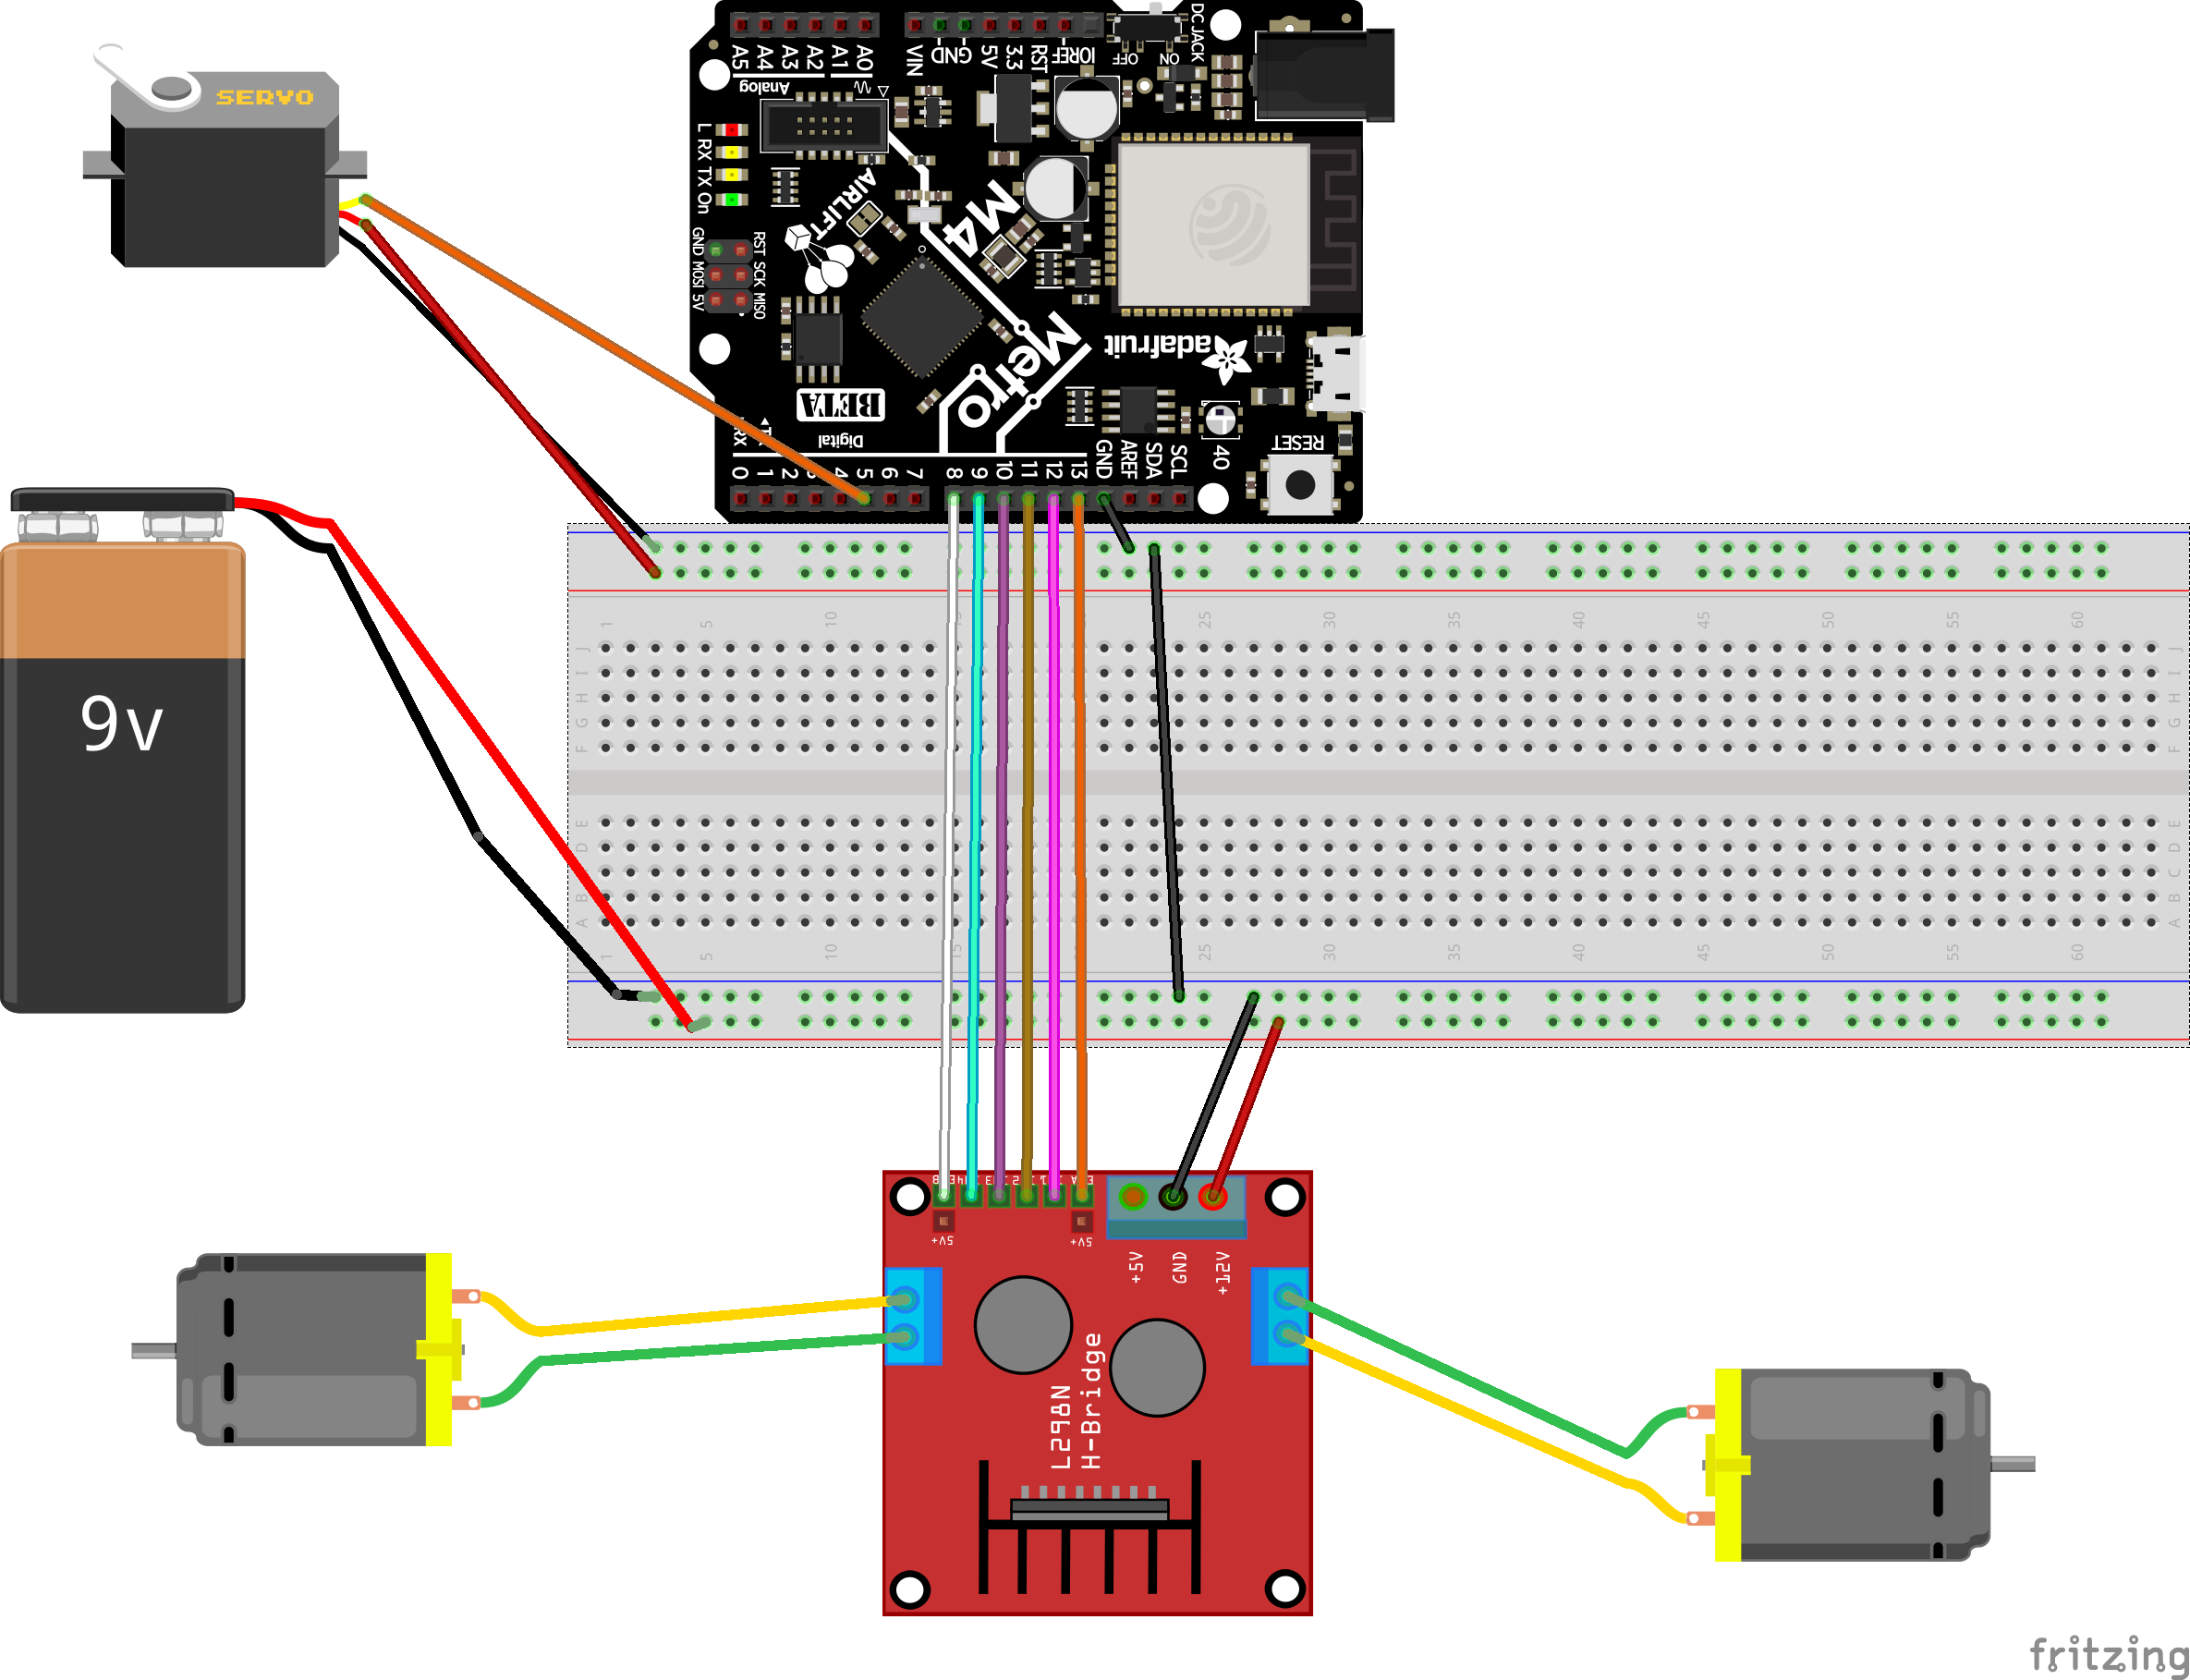
\includegraphics[width=0.8\linewidth]{figures/RC_Boat.png}}
	\caption{Circuit voor het aansturen van een boot}
	\label{fig:RCBoat}
\end{figure}

\newpage

\paragraph{Benodigdheden:}
\begin{itemize}
	\item 1x Servo
	\item 2x DC motor
	\item External power source
	\item 1x L298N H-Bridge Motor Driver
\end{itemize}

\section{Code}
\subsection{Computer client side}
\paragraph{Oplossing:}
\lstinputlisting{code/RCBoat_Client_v2.py}
\paragraph{Discussie:} De code is eigenlijk precies hetzelfde als recept~\ref{sub:KeyboardServoClient}. Er is weer de key\_handler() functie die wordt aangeroepen bij een keyboard event. De functie stuurt het event door naar de key\_press\_handler() als een toets is ingedrukt en naar de key\_release\_handler als een toets is losgelaten. Er is de functie sendData() voor het coderen en sturen van data en een functie checkStateChange() om te controleren of er een verandering is ten opzichte van de laatst gestuurde richting. Het enige verschil is dat de PACK\_DICT, button\_state en functies uitgebreid zijn met de "up" en "down" toetsen. Als de code niet duidelijk is lees dan recept~\ref{sub:KeyboardServoClient} nog een keer.

\newpage
\subsection{Boat server side}
\paragraph{Oplossing:}
\lstinputlisting{code/RCBoat_Server_v2.py}
\paragraph{Discussie:} Deze code is een combinatie van recept~\ref{sec:DC_Servo_Toeter_Joystick} en recept~\ref{sub:KeyboardServoServer}. Eerst worden imports en definities gedaan. Daarna wordt de DC\_motor() class gedefinieerd die is hergebruikt van recept~\ref{sec:DC_Servo_Toeter_Joystick}. 
Na de definities worden de servo, dc motoren en het netwerk ge\"initialiseerd en gaat het programma de oneindige while loop in. Zodra het een connectie heeft leest het de gestuurde data uit, converteert de data naar een string, haalt de laatst gestuurde character uit de string en zoekt de bijbehorende tuple op in de dictionary. Vervolgens wordt de tuple en uitgepakt in een rudderAngle en een motorvalue die tot slot worden gebruikt om de servo en motoren in te stellen. 






